\chapter{Method Details}

\section{Record Linkage}
\label{sec:record-linkage-appendix}

The Jaro-Winkler formula is defined in two steps. First, The Jaro distance, $d_j $, is defined as:

% good code-based illustration at: http://www.gettingcirrius.com/2011/01/calculating-similarity-part-2-jaccard.html

\begin{equation}
  d_j = \left\{
  \begin{array}{l l}
    0 & \text{if }m = 0 \\ 
    \frac{1}{3}\left(\frac{m}{|s_1|} + \frac{m}{|s_2|} + \frac{m-t}{m}\right) & \text{otherwise} \end{array} \right.
\end{equation}

Where:\\
m = number of matching patterns \\
t = number of transposed characters \\
|s1| = length of first string \\
|s2| = length of second string \\

Two characters are considered matching when they are no further apart than:
\begin{equation}
  \left\lfloor\frac{\max(|s_1|,|s_2|)}{2}\right\rfloor-1
\end{equation}

The second component, added by Winkler, preferentially weights strings which match from the beginning, set by the prefix length $ l $.  Thus, the Jaro-Winkler distance is defined:

\begin{equation}
  d_w = d_j + (\ell p (1 - d_j))
\end{equation}

Where $ p $ is a constant scaling factor to adjust for the strength of common prefixes. In its usage here, $ p = 0.1 $ and $ l = 4 $.


\section{Observation Filtering}
% XXX oliver: Cool, power-law, but how exactly do you use this to filter?  Is there more than just screening by the theoretical maximum?
As in many large datasets, the distribution of observations per ship follows an approximate power-law distribution. Using the raw number of observations received in our 15 month window provides a simple filter. The peak in the kernel density estimation (Figure \ref{fig:obs-per-vessel-log}) is seen around $10^4$ observations, with a clear drop-off after $10^5$, which is consistent with the theoretical maximum (one observation in every sample) of about $6.8 \times 10^5$.
\begin{figure}[htbp]
  \centering
  \includegraphics[width=120mm]{figures/obs-per-vessel-log-qplot.pdf}
  \caption[Observations per vessel]{Observations per vessel, kernel density estimation.}
  \label{fig:obs-per-vessel-log}
\end{figure}

\section{Movement Modeling}
\label{sec:movement-modeling-appendix}

% XXX From Jano: provide more detail on what actually was done. Code, whatever, fine -- but include details. It can be in an appendix, but need to include information like cell size, processing techniques, and other details of what the heck you actually did. [Move some stuff from the methods into this appendix].

After storing the raw observations in a spatial database (PostGIS), I used parallelized code to quickly aggregate the large volume of observations. Taking advantage of the database, observations were ordered on disk based on vessel, and spatial indices were created. This allows us to quickly filter the data both based on attributes and spatial traits.

To rasterize vessel tracks, \textsf{gdal\_rasterize} from \textsf{GDAL} was used to convert between vector and raster representations.  Bresenham's line algorithm~\cite{bresenham1965} determined the output cells considered used within each track. I only counted a ship moving through a single cell a single time to capture overall movement patterns, but future work should also incorporate total trips to capture movement patterns such as regular short distance trips passenger ferries engage in. When combining the data, a parallelized version of Matthew Perry's \textsf{gdal\_add.py} script was used to quickly combine thousands of raster ship tracks.

\chapter{Tables}

\begin{table}[htbp]
  \caption[AIS broadcast attributes]{AIS broadcast attributes. Update frequency depends on ship speed, but varies between a minimum of a record every 2 seconds for quickly moving vessels, to once per 3 minutes for moored vessels. Additional attributes are available, but infrequently used.}
  \begin{tabular}{lr}
    \hline
    Attribute & Accuracy \\
    \hline
    Location (fixed from GPS signal) & $\simeq$10 meter \\
    Timestamp (on broadcast) & $\pm100$ ms \textit{transmission \& processing}\\
    Name \\
    Call Sign \\
    Maritime Mobile Service Identity \\
    Heading \\
    Speed \\
    Destination & \textit{often incorrect}
  \end{tabular}
  \label{table:ais-broadcast-attributes}
\end{table}

% table describing the record linkage technique used for each data source
% SOURCE: record-linkage/FRIL/config/*.xml
\begin{table}[htbp]
  \caption[Ship record linkage methods]{Ship record linkage methods used.}
  \ssp
  \renewcommand{\arraystretch}{1.4}
  \begin{tabular}{rrrlrr}
    \hline
    Source $A$ & Source $B$ & acceptance level & column & distance metric & weight \\
    \hline
     DS & ITU & 92 & callsign & Jaro-Winkler\textsuperscript{1} & 50 \\
        &     &    & MMSI & equal & 40 \\
        &     &    & name & Jaro-Winkler & 40 \\
    \hline
     DS &  VT & 85 & callsign & Jaro-Winkler & 60 \\
        &     &    & IMO & Jaro-Winkler & 20 \\
        &     &    & name & Jaro-Winkler & 20 \\
    \hline
    FCC & ITU & 85 & callsign & Jaro-Winkler & 95 \\
        &     &    & name & Jaro-Winkler & 5 \\
    \hline
    FCC &  VT & 95 & callsign & Jaro-Winkler & 66 \\
        &     &    & name & Jaro-Winkler & 5 \\
        &     &    & MMSI & Jaro-Winkler & 24 \\
        &     &    & length & equal & 5 \\
    \hline
     VT & ITU & 80 & callsign & Jaro-Winkler & 20 \\
        &     &    & MMSI & Edit Distance & 30 \\
        &     &    & name & Jaro-Winkler & 10 \\
        &     &    & IMO & Jaro-Winkler & 40 \\
    \hline
     DS & FCC & 95 & callsign & equal & 99 \\
        &     &    & name & Jaro-Winkler& 1 \\
  \end{tabular}
  \\
  \\
  1. Jaro-Winkler distance \citep{winkler1990string}: length $l = 4$ and scaling factor $p = 0.1$
  \label{table:ships-record-linkage-methods}
\end{table}


% had this as a list, also some hackery with unnesting class data:
% select distinct(trim(both from unnest(class))), count(*) from clean.ships where validation_class = 'tanker' and validation_score > 0 and obs_count > 0 GROUP BY class ORDER BY btrim DESC;ships=# select distinct(trim(both from unnest(class))), count(*) from clean.ships where validation_class = 'tanker' and validation_score > 0 and obs_count > 0 GROUP BY class ORDER BY btrim DESC;
\begin{longtable}{l|l|l}

\hline \multicolumn{1}{|c|}{\textbf{Type}} & \multicolumn{1}{c|}{\textbf{Sub-type}} & \multicolumn{1}{c|}{\textbf{Vessels}} \\ \hline 
\endfirsthead
%\multicolumn{3}{c}%
%{{\bfseries \tablename\ \thetable{} -- continued from previous page}} \\
\hline \multicolumn{1}{|c|}{\textbf{Type}} &
\multicolumn{1}{c|}{\textbf{Sub-type}} &
\multicolumn{1}{c|}{\textbf{Vessels}} \\ \hline 
\endhead

%\hline \multicolumn{3}{|r|}{{Continued on next page}} \\ \hline
\endfoot
    cargo & cargo ship & 30355 \\
          & merchant & 2919 \\
          & bulk carrier & 1338 \\
          & container ship & 669 \\
          & general cargo & 608 \\
          & vehicle carrier & 56 \\
    tanker & tankship & 10460 \\
           & tanker   & 8731 \\
           & oil tanker & 1312 \\
           & liquefied gas carrier & 112 \\
           & chemical carrier & 39 \\
    other & merchant & 17460 \\
          & other ship & 9421 \\
          & unspecified & 4580 \\
          & motor boat & 4231 \\
          & inland waterways & 3825 \\
          & sloop & 2799 \\
          & reserved for future use & 2164 \\
          & all other activities & 1345 \\
          & reserved for regional use & 712 \\
  support & pusher/tug & 4392 \\
          & tug & 7885 \\
          & towing vessel & 2747 \\
          & supply vessel & 1501 \\
          & service vessels & 1388 \\
          & trawler & 1056 \\
          & dredger & 995 \\
          & vessel engaged in dredging or underwater operation & 776 \\
          & pilot vessel & 685 \\
  pleasure & pleasure/leisure & 22013 \\
           & pleasure & 14573 \\
           & pleasure craft & 7290 \\
           & sailing vessel & 5527 \\
           & yacht & 8214 \\
  fishing & fishing vessel & 11110 \\
          & fishing boat & 8454 \\
          & fishing industry & 5767 \\
          & fishing & 3213 \\
  passenger & passenger ship & 6478 \\
            & ferry & 704 \\
  high-speed & high-speed craft & 658 \\
             & high speed craft & 520 \\
  authority & sar-vessel & 699 \\
            & search and rescue vessel & 609 \\
            & rescue vessel & 102 \\
  \caption[Detailed ship classes]{Detailed ship classes, derived from observations.}
  \label{table:ship-class-breakdown}
\end{longtable}

\chapter{Software}
\label{sec:software}

% include SOME python code here -- our AIS parser, what else?
% steps: download AIS
% parse AIS
% insert AIS into DB, formalize
% download & parse ship databases

This work would not have been possible without extensive contributions from others in the form of software, both commercial and open source. An overview of the software used in the project is provided, and code produced is available at \url{https://github.com/scw/thesis}. 

To store the raw observations, \textsf{SQLite} was used for rapid development, but the bulk of the observations were stored in the object-relational database \textsf{PostgreSQL}, where analysis was carried out using either native SQL or with the spatial extension \textsf{PostGIS}. The \textsf{GDAL} library was used extensively for transforming both raster and vector data, and aggregation. Record linkage was performed using \textsf{FRIL}, with some record linkage integrated into the database using \textsf{pg\_similarity}, and in \textsf{Python} using the \textsf{jellyfish} module. Integration and data processing used \textsf{Python}, which combines a wide base of environments within a single language. \textsf{R} was used to perform statistical analyses and summarize results. \textsf{GRASS} was used to compute model outputs and spatial statistics, and maps were produced in \textsf{ArcGIS} and \textsf{Quantum GIS}.

\begin{table}[htbp]
  \caption[Software used]{Software used. A complete listing of software packages used in the analysis.}
  \ssp
  \centering
  \begin{tabular}{rr}
    \hline
    Software package & version \\
    \hline
     \textsf{ArcGIS} & 10.1 \\
     \textsf{Bash} & 4.2.24 \\ 
     \textsf{FRIL} & 2.1.5 \\
     \textsf{GDAL} & 1.8.0 \\
                 " & 1.9.1 \\
                 " & 1.9.2 \\
     \textsf{Git} & 1.7.9.5 \\
     \textsf{GRASS} & 6.4 \\
                  " & 7.0 \\
     \textsf{pg\_similarity} & 0.0.19 \\
     \textsf{PostGIS} & 1.5.3 \\
                    " & 2.0.1 \\
     \textsf{PostgreSQL} & 8.4.14 \\
                      "  & 9.2.1 \\
     \textsf{Python} & 2.6 \\
                   " & 2.7.2 \\
     \textsf{Quantum GIS} & 1.8 \\
     \textsf{R} & 2.14 \\
              " & 2.15 \\
     \textsf{SQLite} & 3.7.9 \\
  \end{tabular}
  \label{table:software-used-versions}
\end{table}

\begin{table}
  \caption[Libraries used]{External libraries used. Python was used extensively throughout the project, and R was used for calculations, validation, and statistics. The following external libraries were used in each environment.}
  \centering
  \ssp
  \begin{tabular}{ll}
    \hline
    R packages & Python libraries \\
    \hline
    foreign & BeautifulSoup\\
    geosphere & gdal \\
    ggplot2 & geographiclib \\
    maptools & geojson \\
    plotrix & geopy \\
    raster & grass\\
    RPostgreSQL & jellyfish \\
    rgdal & numpy \\
    rgeos & ogr \\
    sm & psycopg2 \\
    sp & requests \\
  \end{tabular}
\end{table}

\chapter{Figures}
\label{sec:figures}

\begin{figure}[htbp]
  \centering
  \hspace*{-.3in}
  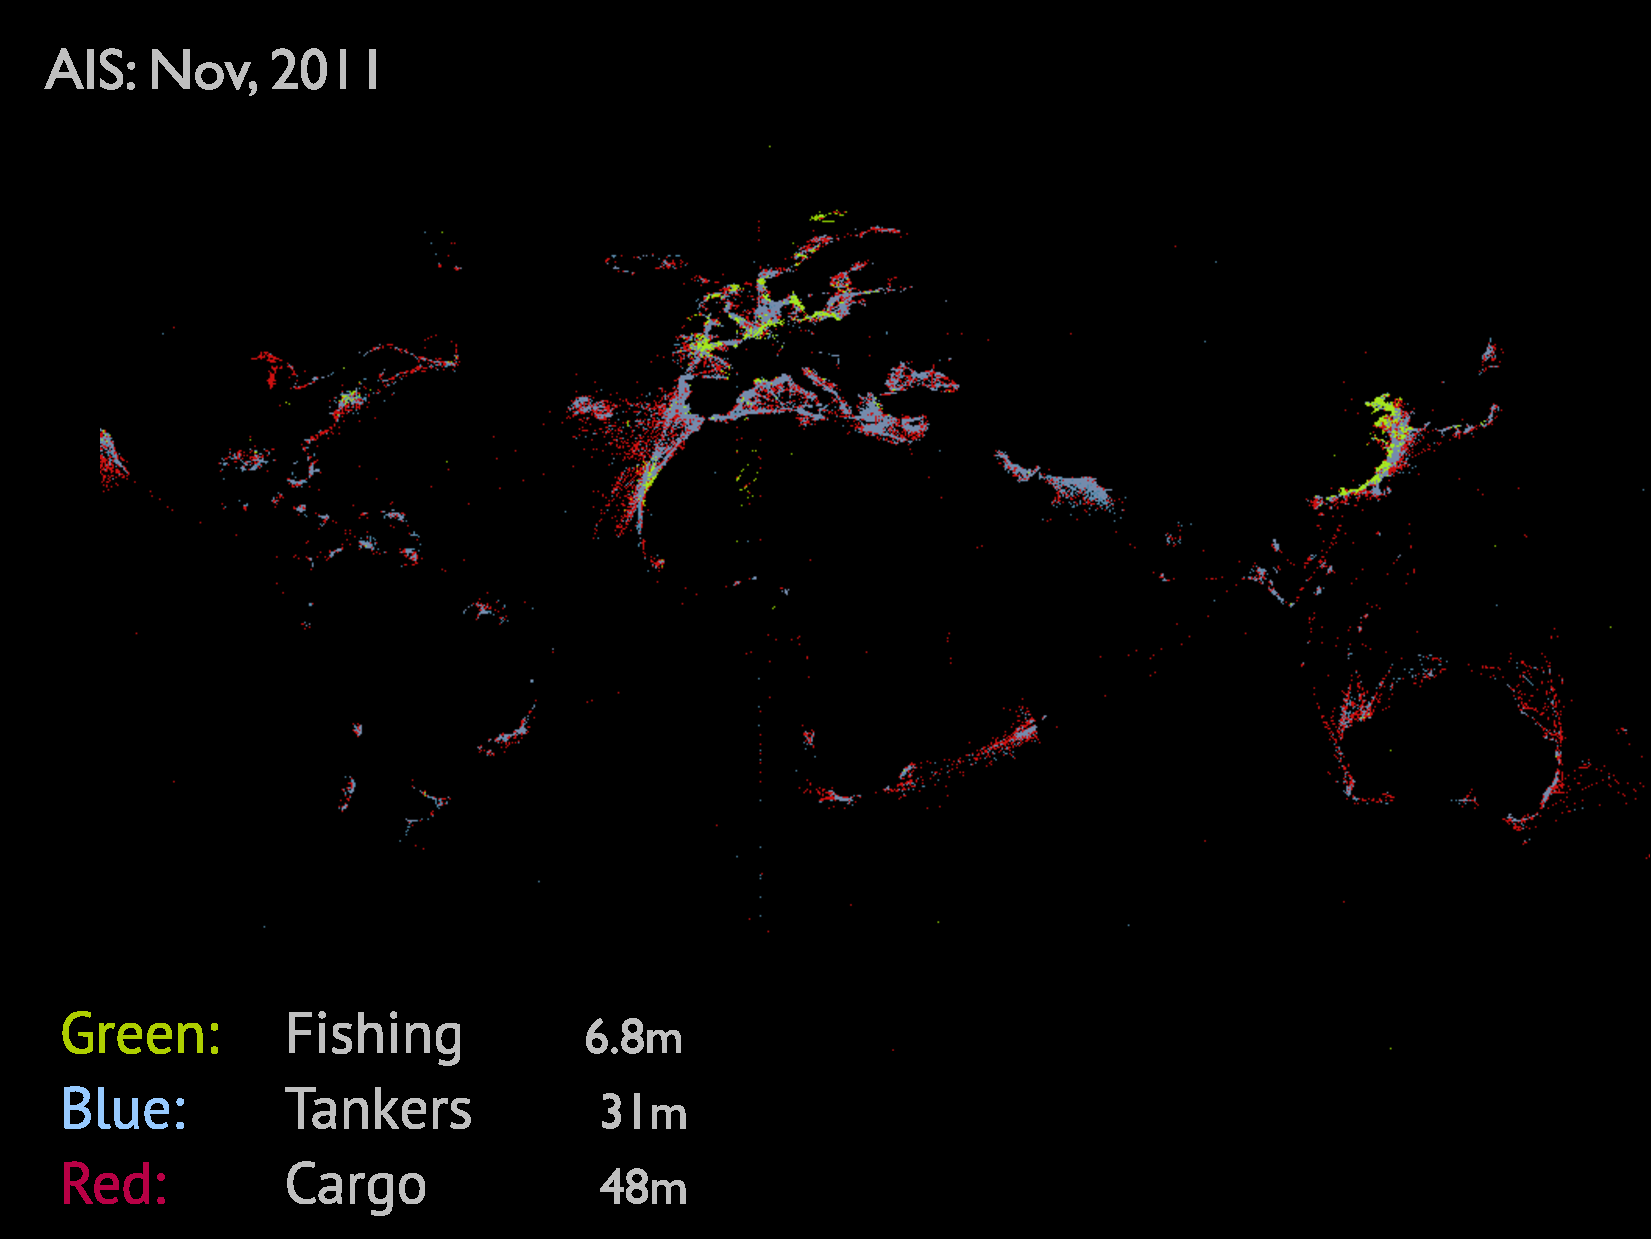
\includegraphics[width=140mm]{figures/ais-nov-2011.pdf}
  \caption[AIS observations, November 2011]{Raw AIS observations, November 2011. Note the observations located in the Hoggar Mountains in Algeria.}
  \label{fig:ais-obs-nov-2011}
\end{figure}

\begin{figure}
  \centering
  \hspace*{-.3in}
  \includegraphics[width=120mm]{figures/ais-and-ports-cea.pdf}
  \caption[AIS coverage]{Approximate AIS coverage (green), global ports (red).}
  \label{fig:ais-coverage}
\end{figure}

% show our image of invalid 'on land' ships in the harbor of long beach?
\begin{figure}
  \centering
  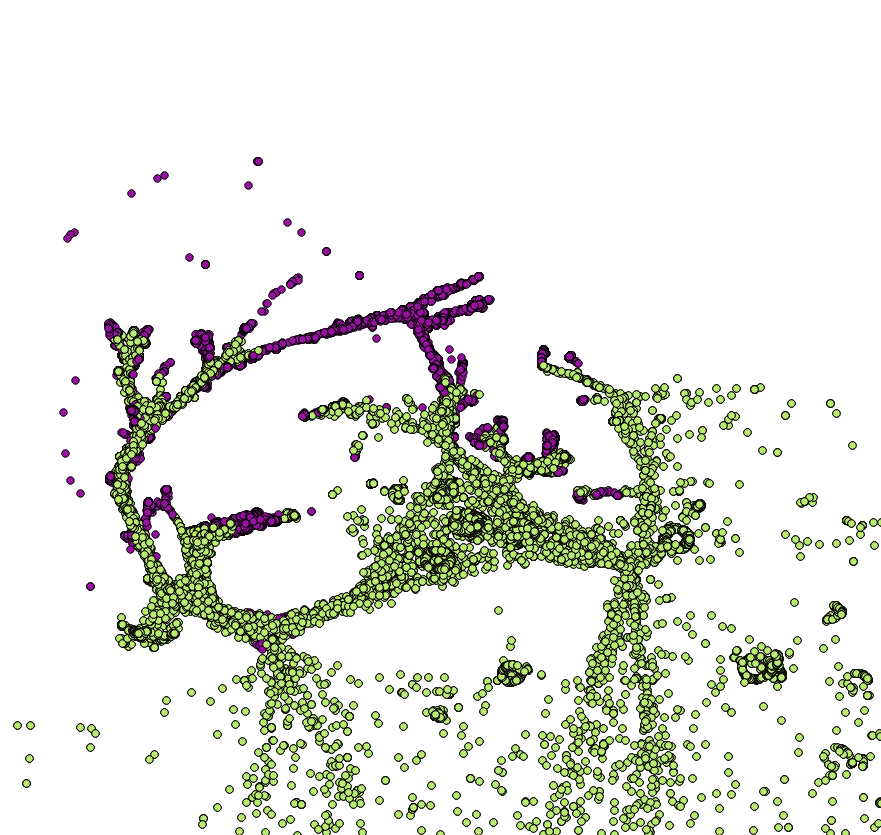
\includegraphics[width=120mm]{figures/example-long-beach-harbor-validation.png}
  \caption[Long Beach harbor, validation]{Long Beach Harbor, California. Points shown in purple are 'on land', but most of these observations are actually within the harbor.} % XXX Oliver: a little context here?
  \label{fig:longbeach-validation}
\end{figure}

\begin{figure}[htbp]
  \centering
  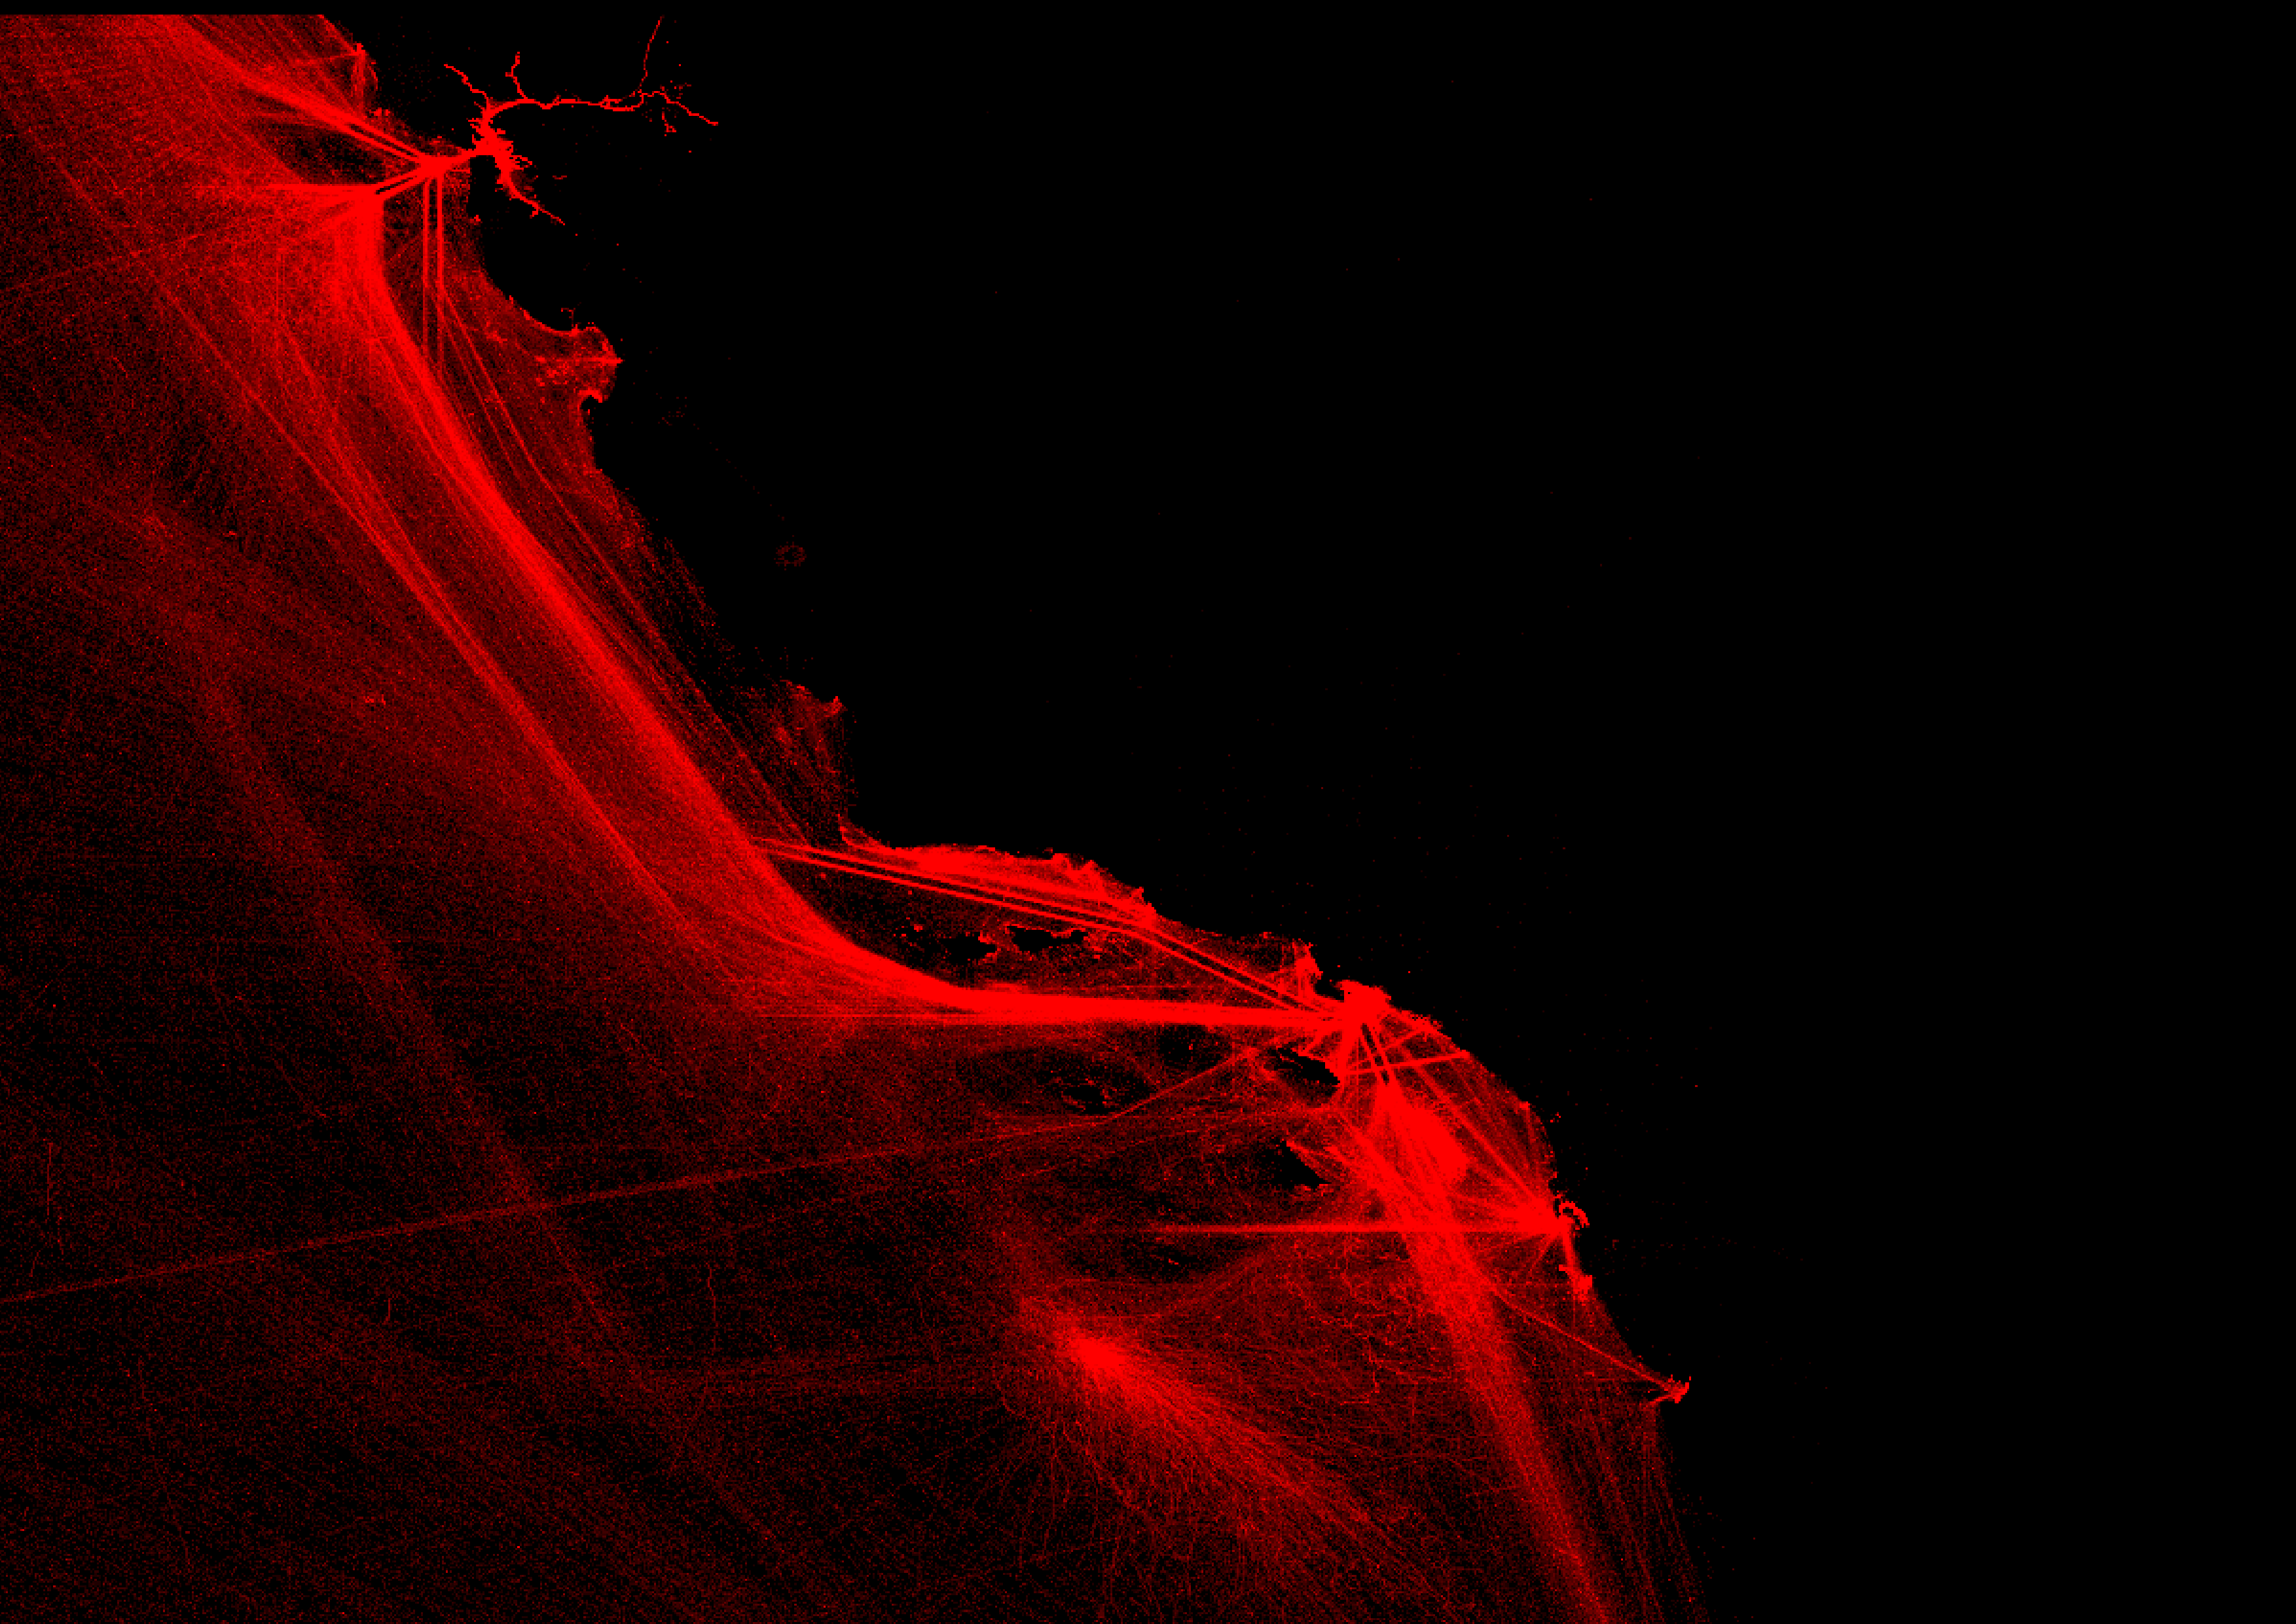
\includegraphics[width=140mm]{figures/cargo_density.png}
  \caption[AIS observations, Southern California Bight]{AIS observations, Southern California Bight. Nov 2010--Dec 2011. Note the ballast water exchange point lower left.}
  \label{fig:cal-cargo}
\end{figure}

\begin{figure}[htbp]
  \centering
  \hspace*{-.15in}
  \includegraphics[width=150mm]{figures/cia-lanes-small-cropped.png}
  \caption[CIA "World Shipping Lanes"]{"World Shipping Lanes" map produced by the Central Intelligence Agency, 1973.}
  \label{fig:cia-shipping-map}
\end{figure}


